\subsection{Meet Chef}

\frame
{
  \frametitle{Meet Chef}

  \begin{center}
    \Huge Meet Chef
  \end{center}
}

\frame
{
  \frametitle{Meet Chef}

  \begin{itemize}
  \item<1-> Configuration Management
  \item<2-> HTTP(S) Client/Server based
  \item<3-> Erlang Server
  \item<4-> Ruby client
  \end{itemize}
}

\frame
{
  \frametitle{Chef Infrastructure}
  \begin{center}%
    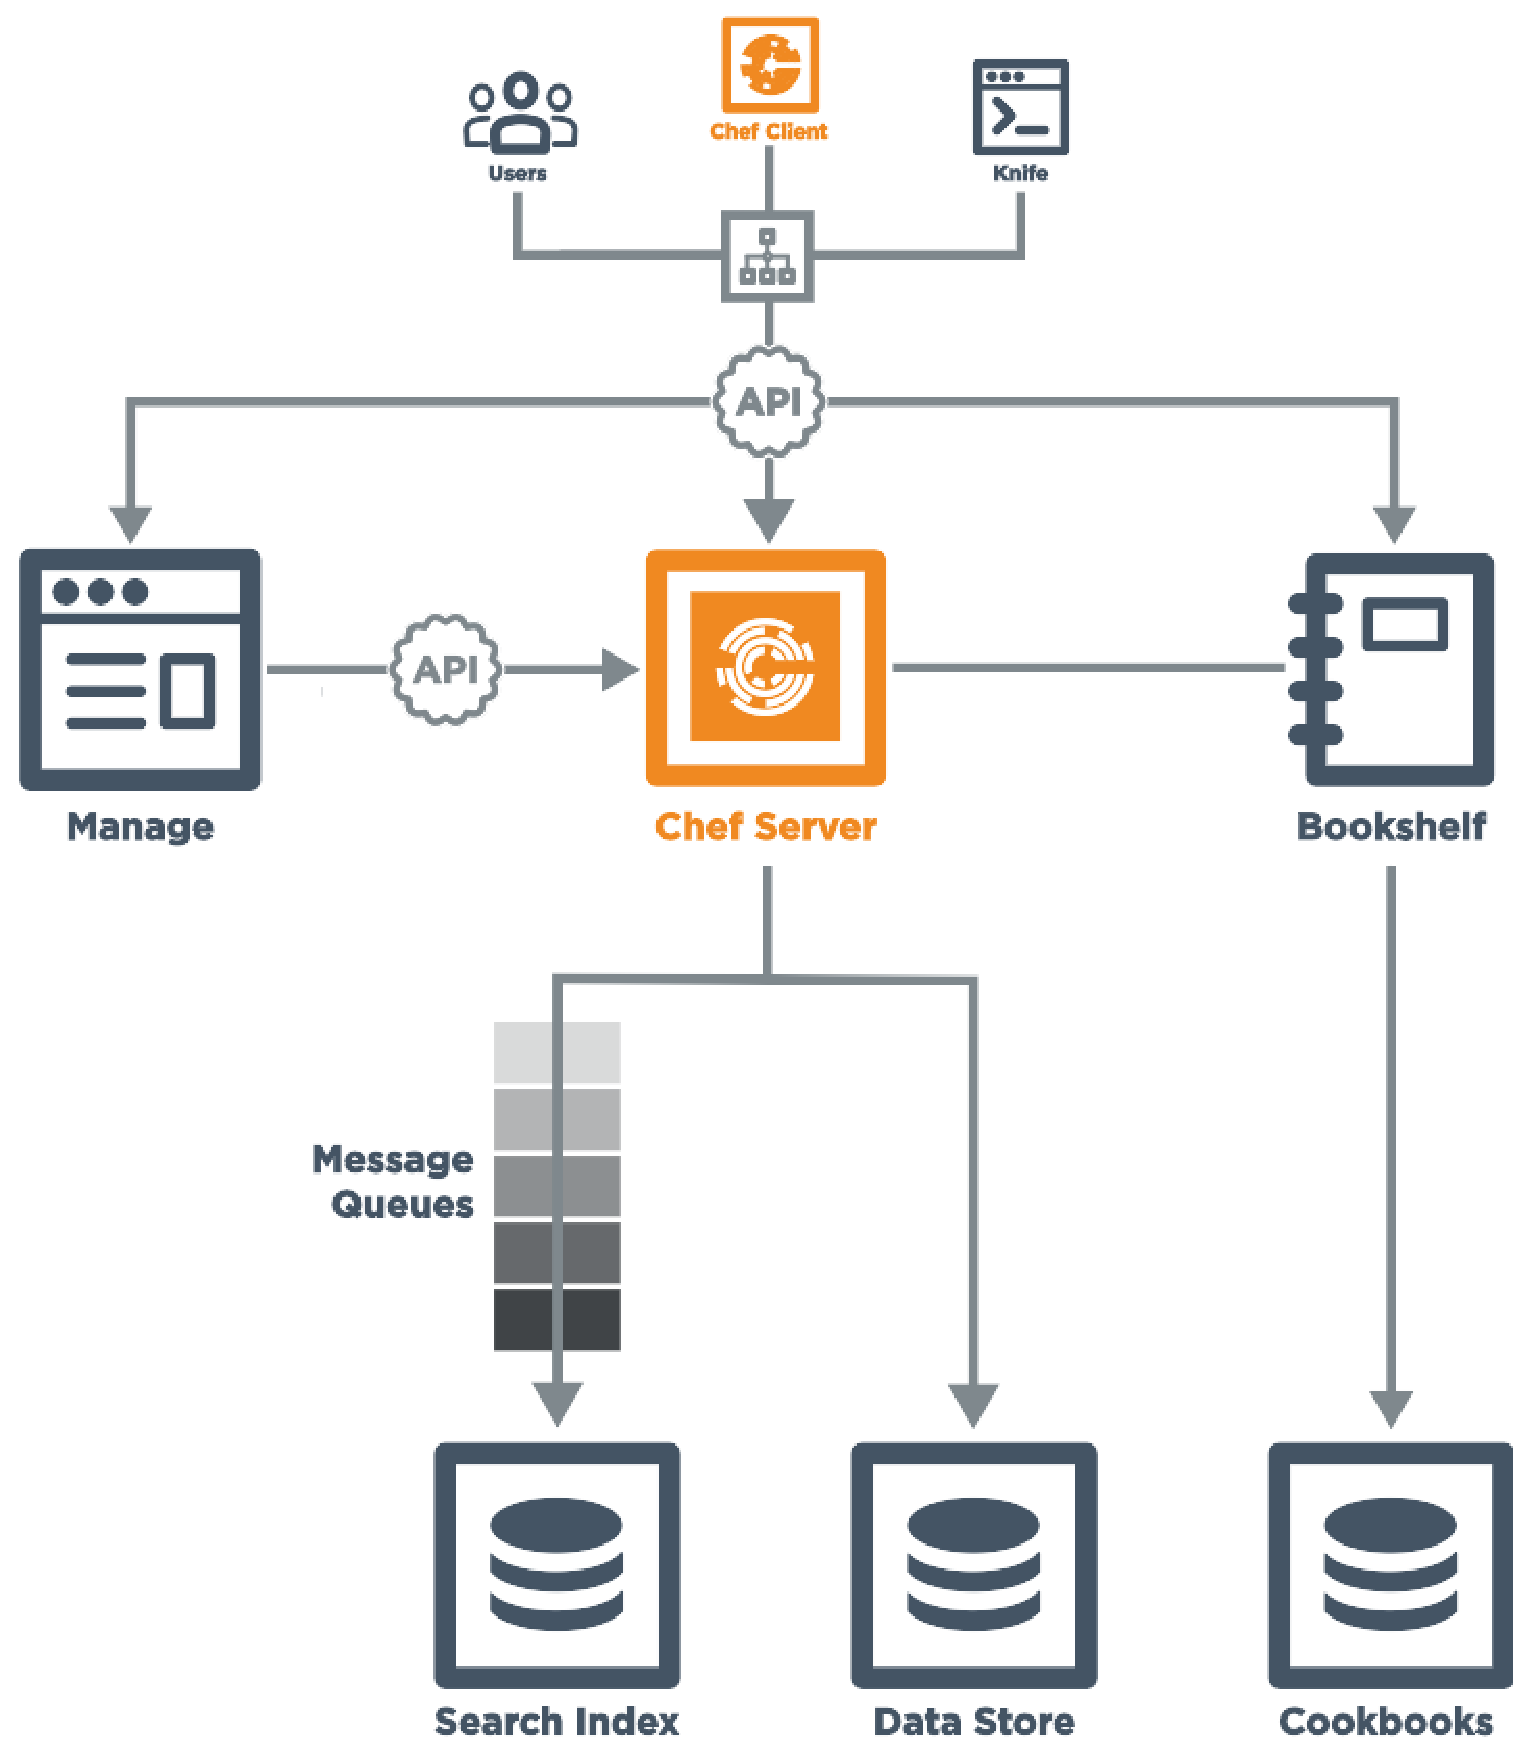
\includegraphics[height=6cm]{images/server_components.pdf}
  \end{center}%
}

\frame
{
  \frametitle{Learning Chef}

  \begin{itemize}
  \item<1-> Start with Chef Solo/Zero
  \item<2-> Ruby DSL
  \end{itemize}
  \includegraphics<3->[scale=0.5]{images/recipe.png}
}

\frame
{
  \frametitle{Chef Basic Concepts}

  \begin{itemize}
  \item<1-> Cookbooks
  \item<2-> Recipies
  \item<3-> Nodes
  \item<4-> Clients
  \item<5-> Roles
  \item<6-> Environments
  \end{itemize}
}

\frame
{
  \frametitle{Setting up Chef}

  \begin{itemize}
  \item<1-> Standalone/Hosted
  \item<2-> Bootstrap script
  \item<3-> HTTPS - Certificate
  \item<4-> CLI tools serverside
  \item<5-> CLI tools client side
  \end{itemize}
}

\frame
{
  \frametitle{Bootstrapping a node}

  \begin{itemize}
  \item<1-> Install embedded ruby
  \item<2-> Install chef (gem)
  \item<3-> Set up credentials
  \item<4-> Run chef-client first time
  \end{itemize}
}

\subsection{Becomming a chef}
\frame
{
  \frametitle{Cookbook structure}

  \begin{itemize}
  \item knife cookbook create foobar
  \end{itemize}
  \begin{center}
  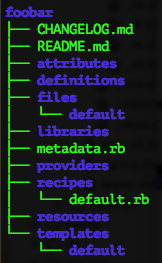
\includegraphics[scale=0.5]{images/cookbook_structure.png}
  \end{center}
}

\frame
{
  \frametitle{Applying a cookbook}

  \begin{itemize}
    \item knife cookbook upload foobar
    \item knife node run\_list add foobar.example.com 'recipe[foobar]'
    \item Wait for chef-client to run - defaults to every 30 minutes
  \end{itemize}
}

\frame
{
  \frametitle{Community Resources}

  \begin{itemize}
    \item supermarket.chef.io
    \item Berkshelf
    \item Open Source chef cookbooks (Facebook, Riot Games, etc.)
    \item "Chef Style DevOps Kungfu"
  \end{itemize}
}

\subsection{Summary}
\frame
{
  \frametitle{Overall thoughts}

  \begin{itemize}
    \item<1-> Rather complex
    \item<2-> Convention over Configuration
    \item<3-> Conventions are necessary
    \item<4-> "Round Trip Time" is rather large
    \item<5-> Well tested
    \item<6-> Test Kitchen
    \item<7-> Proven in large setups (30k+ nodes)
    \item<8-> Scaling is a "Black art"
  \end{itemize}
}

